\chapter{Contesto di svolgimento delle attività}
\label{cap:contesto-svolgimento}

Questo capitolo si occupa di fornire informazioni in merito a \textit{\textbf{Trizeta}}, azienda ospitante del tirocinio, al settore in cui essa opera (quindi anche ai beni e servizi offerti), 
al suo rapporto con l'introduzione di novità / con il miglioramento di processi e strumenti già in uso ed ai processi in essa utilizzati. \\
Le informazioni riportate di seguito sono frutto di osservazioni personali, dialoghi avuti nel corso del tirocinio e ricerche svolte in totale autonomia.

\section{Introduzione all'azienda ospitante}

% In questa sezione descriverò brevemente l'azienda, indicandone dimensioni, ubicazione, figure presenti all'interno dell'organico, gruppo commerciale di cui fa parte.
\textit{\textbf{Trizeta}} è una \textit{software house}\footnote{\gls{software-house}}, ovvero un'azienda che si occupa dello sviluppo e della commercializzazione di \textit{software}, specializzata nella consulenza e nello sviluppo
di prodotti per aziende che desiderano l'automazione (totale o parziale) delle proprie attività industriali (compresa la gestione del magazzino); essa consente inoltre alle aziende clienti di gestire le proprie risorse digitali multimediali (i cosiddetti \textit{digital assets}\footnote{\gls{digital-asset}}).
\vspace{-20mm}
    \begin{figure}[H]
        \centering
        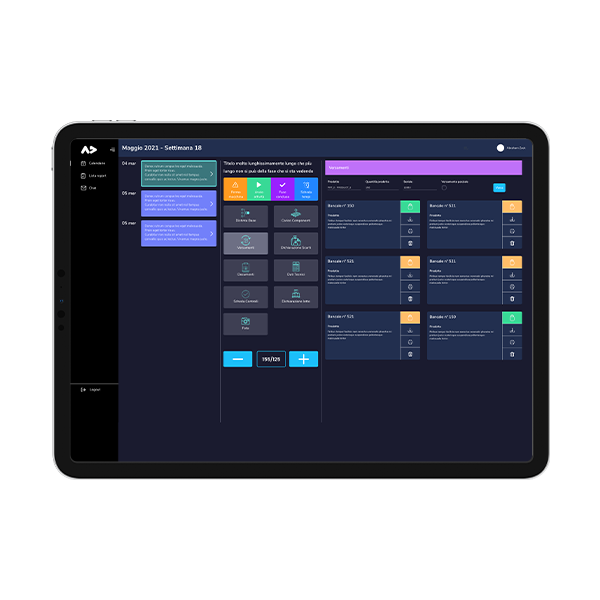
\includegraphics[width=0.7\textwidth]{images/adesuite.png}
        \vspace{-15mm}
        \caption[Caption for LOF]{Interfaccia di un gestionale \textit{\textbf{Trizeta}}\footnotemark}
    \end{figure}
    \footnotetext{Fonte: \href{https://trizeta.com/ade-mes/}{https://trizeta.com}}

L'azienda è ubicata a \textit{Monselice (Padova)} e dispone all'incirca di una decina di dipendenti \textit{IT}\footnote{\gls{it}} (informatici) tra loro eterogenei per anni di esperienza nel settore informatico, età anagrafica, e 
\textit{stack} tecnologico\footnote{\gls{tech-stack}} abitualmente utilizzato (tecnologie utilizzate e ambito di utilizzo delle stesse). \\
Recentemente \textit{\textbf{Trizeta}} è entrata a far parte di \textit{SYS-DAT Group}: è un gruppo di aziende specializzate nello sviluppo e manutenzione di prodotti \textit{software} rivolti ad aziende appartenenti a vari settori quali 
il settore moda (settore di origine di \textit{SYS-DAT}, azienda fondatrice del gruppo) ed il settore alimentare. 


\section{Prodotti e servizi}

% In questa sezione descriverò brevemente i prodotti ed i servizi offerti dall'azienda che ho potuto vedere (mi focalizzerò su un prodotto in particolare, dato che il software che ho prodotto nel corso del tirocinio andrà ad essere integrato con esso).
% Terminerò la sezione indicando la clientela a cui l'azienda si rivolge.
Come già indicato nella sezione precedente, \textit{\textbf{Trizeta}} intrattiene relazioni commerciali esclusivamente di tipo \textit{B2B}\footnote{\gls{b2bg}}: questa visione si riflette inevitabilmente sui prodotti offerti
e sull'insieme dei requisiti utente soddisfatti dai prodotti commercializzati. \\
Di seguito, un breve elenco di software che ho potuto visionare personalmente e, relativamente all'ultima voce in lista, studiare ai fini di comprendere meglio le finalità dello \textit{stage} e la visione dell'azienda:

\begin{itemize}
    \item \textit{ADeWMS}: è un \textit{WMS}\footnote{\gls{wmsg}} (gestionale relativo al contenuto e alle attività di magazzino) in grado di integrarsi con software \textit{ERP}\footnote{\gls{erpg}} e gestire ordini commerciali, consegne e relativa documentazione;
    \begin{figure}[H]
        \centering
        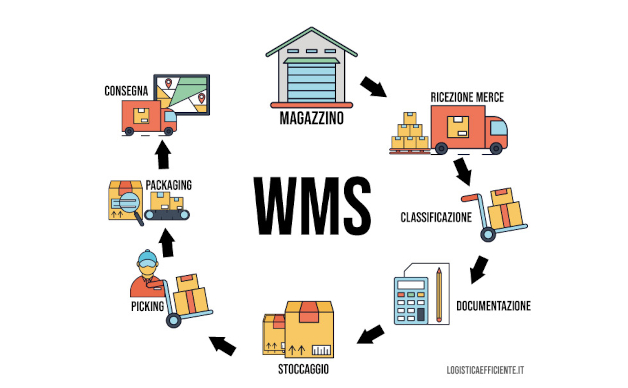
\includegraphics[width=0.9\textwidth]{images/wms.jpg}
        \caption[Caption for LOF]{Attività gestite da un \textit{software \glslink{wmsg}{WMS}} \footnotemark}
    \end{figure}
    {\footnotetext{Fonte: \href{https://www.logisticaefficiente.it/wiki-logistica/magazzino/wms-warehouse-management-system.html}{https://www.logisticaefficiente.it}}}
    
    \item \textit{P4NDOR4}: è un \textit{DAM}\footnote{\gls{damg}} (gestionale per \glslink{digital-asset}{\textit{digital assets}} aziendali) con possibilità di richiedere delle risorse direttamente a \textit{\textbf{Trizeta}};
    \begin{figure}[H]
        \centering
        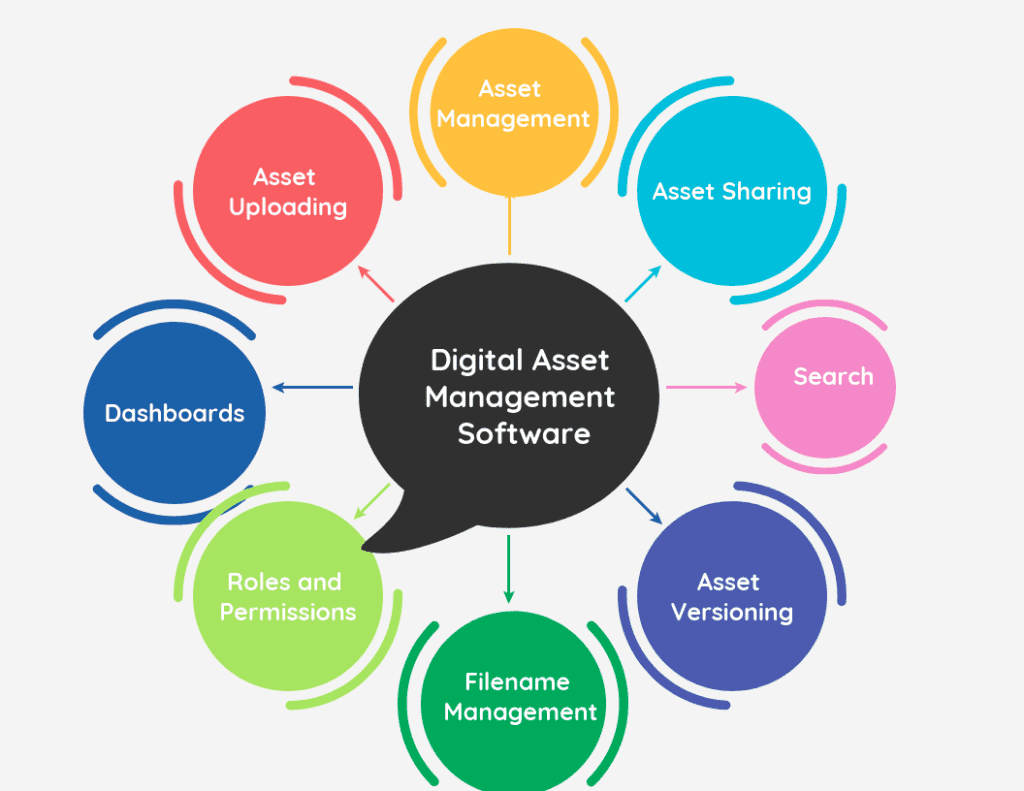
\includegraphics[width=0.85\textwidth]{images/dam.png}
        \caption[Caption for LOF]{Funzionalità di un \textit{software \glslink{damg}{DAM}} \footnotemark}
    \end{figure}
    {\footnotetext{Fonte: \href{https://vitolavecchia.altervista.org/che-cose-come-funzione-e-vantaggi-della-gestione-delle-risorse-digitali-dam-in-informatica/}{https://vitolavecchia.altervista.org/}}}

    \item \textit{ADeMES}: è un \textit{MES}\footnote{\gls{mesg}} (\textit{software} di gestione delle attività produttive aziendali) di particolare interesse in quanto direttamente coinvolto ai fini del tirocinio.
    \begin{figure}[H]
        \centering
        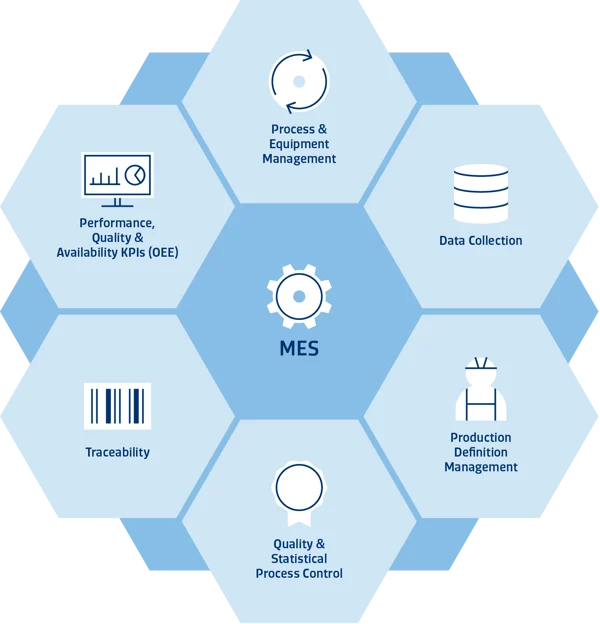
\includegraphics[width=0.55\textwidth]{images/mes.png}
        \caption[Caption for LOF]{Funzionalità di un \textit{software \glslink{mesg}{MES}} \footnotemark}
    \end{figure}
    {\footnotetext{Fonte: \href{https://www.systema.com/blog/build-or-buy-your-next-mes}{https://www.systema.com}}}

    \textit{ADeMES} è dotato delle seguenti caratteristiche (rilevanti ai fini del tirocinio):
    \begin{itemize}
        \item Presenza di un'area personale per ogni operatore (lavoratore in linea di produzione);
        \item Lista di "fasi" di lavorazione attive (schedulate o in esecuzione);
        \item Possibilità di allegare documenti e note testuali ad ogni fase di lavorazione attiva; queste funzionalità hanno molteplici scopi e, tra questi, vi era anche la registrazione di dati di qualità prima dell'inizio del periodo di tirocinio.
    \end{itemize}
\end{itemize}

\section{Processi interni}

Il \textit{team} aziendale utilizza un modello di ciclo di vita del software detto \textit{agile}, ovvero ha una visione orientata all'ottimizzazione del flusso di lavoro (evitando tempi morti e uso di risorse senza ottenere valore in cambio), 
e consentire una risposta rapida alle variazioni delle esigenze del cliente anche in stadi avanzati dello sviluppo \footnote{\hyperref[app:agile]{Appendice: metodologie agili}}.

% In questa sezione descriverò ciò che ho potuto osservare nel periodo di tirocinio relativamente alle attività lavorative degli altri dipendenti IT, descrivendo il supporto ricevuto in relazione al mio tirocinio.
\begin{itemize}
    \item \textbf{Gestione di progetto}: in relazione alla gestione di progetto, ho potuto assistere (direttamente o indirettamente) alle seguenti attività:
        \begin{itemize}
            \item \textbf{Definizione degli obiettivi e delle risorse}: la definizione degli obiettivi e delle risorse di progetto avviene dopo dialogo diretto con le industrie clienti coinvolte nel progetto: in questa occasione si cerca di analizzare a fondo 
                i risultati desiderati e le modalità di raggiungimento degli stessi;
            \item \textbf{Pianificazione}: la pianificazione delle attività avviene a partire dalla definizione degli obiettivi e delle risorse di progetto (previo dialogo, come precedentemente indicato), 
                basandosi su esperienze pregresse e sulla disponibilità di capitale umano e risorse economiche;
            \item \textbf{Comunicazione con gli \textit{stakeholders}\footnote{\gls{stakeholder}}}: la comunicazione con i "portatori d'interesse" (coloro i quali hanno interesse nella buona riuscita del progetto) è fondamentale per dare prova di avanzamento tangibile nei modi e tempi indicati o, in caso contrario,
                motivare eventuali discrepanze tra la pianificazione e la realtà.
        \end{itemize}
    \item \textbf{Sviluppo}
        \begin{itemize}
            \item \textbf{Analisi dei requisiti}: l'attività di analisi dei requsiti 
        \end{itemize}
\end{itemize}


\section{Rapporto con l'innovazione}

In questa sezione descriverò quello che, in base alle mie osservazioni e all'esperienza dovuta alle attività di tirocinio, è il rapporto dell'azienda con tutto ciò che riguarda il miglioramento di processi / attività / prodotti già esistenti o l'introduzione di novità.